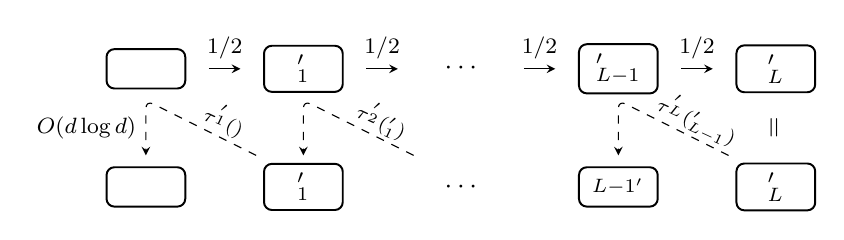
\begin{tikzpicture}
    % Matrices and sampling arrows
    \node [rectangle, line width = 0.25mm, draw, minimum width = 1cm, minimum height = .5cm, rounded corners = 0.1cm]
        (r) at (0,0) {$\A$};

    \draw [-stealth]
        (.8, 0) -- (1.2, 0) node[midway,above] {\footnotesize $1/2$};

    \node [rectangle, line width = 0.25mm, draw, minimum width = 1cm, minimum height = .5cm, rounded corners = 0.1cm]
        (r) at (2,0) {$\A_1'$};

    \draw [-stealth]
        (2.8, 0) -- (3.2, 0) node[midway,above] {\footnotesize $1/2$};
    \node []
        (r) at (4, 0) {$ \cdots $};
    \draw [-stealth]
        (4.8, 0) -- (5.2, 0) node[midway,above] {\footnotesize $1/2$};
    \node [rectangle, line width = 0.25mm, draw, minimum width = 1cm, minimum height = .5cm, rounded corners = 0.1cm]
        (r) at (6,0) {$\A_{L-1}'$};

    \draw [-stealth]
        (6.8, 0) -- (7.2, 0) node[midway,above] {\footnotesize $1/2$};
    \node [rectangle, line width = 0.25mm, draw, minimum width = 1cm, minimum height = .5cm, rounded corners = 0.1cm]
        (r) at (8,0) {$\A_L'$};

    \node [rectangle, line width = 0.25mm, draw, minimum width = 1cm, minimum height = .5cm, rounded corners = 0.1cm]
        (r) at (0,-1.5) {$\B$};

    \node [rectangle, line width = 0.25mm, draw, minimum width = 1cm, minimum height = .5cm, rounded corners = 0.1cm]
        (r) at (2,-1.5) {$\B_1'$};

    \node []
        (r) at (4, -1.5) {$ \cdots $};
    \node [rectangle, line width = 0.25mm, draw, minimum width = 1cm, minimum height = .5cm, rounded corners = 0.1cm]
        (r) at (6,-1.5) {$\B_{L-1'}$};

    \node [rectangle, line width = 0.25mm, draw, minimum width = 1cm, minimum height = .5cm, rounded corners = 0.1cm]
        (r) at (8,-1.5) {$\B_L'$};

    \node [rotate=90]
        (r) at (8, -.75) {$ = $};



    \draw [-stealth, rounded corners = 0.1cm, dashed]
        (1.4, -1.1) -- (0, -.4) -- (0, -1.1) node[midway, left, align=left] {\footnotesize $O(d\log d)$};
    \node [rotate=-25]
        (r) at (1, -.65) {\scriptsize $ \boldsymbol {\tau}^{\B_1'}(\A) $};

    \draw [-stealth, rounded corners = 0.1cm, dashed]
        (3.4, -1.1) -- (2, -.4) -- (2, -1.1) node[midway, left, align=left] {};
    \node [rotate=-25]
        (r) at (3, -.65) {\scriptsize $ \boldsymbol {\tau}^{\B_2'}(\A_1') $};

    \draw [-stealth, rounded corners = 0.1cm, dashed]
        (7.4, -1.1) -- (6, -.4) -- (6, -1.1) node[midway, left, align=left] {};
    \node [rotate=-25]
        (r) at (7, -.65) {\scriptsize $ \boldsymbol {\tau}^{\B_L'}(\A_{L-1}') $};
\end{tikzpicture}